\section{Results}
\label{sec:results}

\subsection{Clean zero-shot performance}
\label{sec:results-clean}

% Source: outputs/studies/final_study/main/results_all.csv (mean/SD) and
% outputs/studies/final_study/main/headline_bootstrap_ci.csv (95% CI, 20,000-repeat
% hierarchical city-then-seed bootstrap -- the SAME construction as every paired-
% comparison CI in this paper; see paper/tables/regenerate_headline_ci.py).
% Regenerate with: python paper/tables/generate_tables.py
\begin{table}[t]
\centering
\caption{Held-out-city results, mean $\pm$ sample SD over nine city--seed runs (3 cities $\times$ 3 seeds), with 95\% bootstrap confidence intervals on the two primary metrics. Bold marks the best mean per column. Note the RUGD/STAEformer intervals overlap on both primary metrics (\Cref{sec:results}).}
\label{tab:headline}
\resizebox{\linewidth}{!}{%
\begin{tabular}{lccccc}
\toprule
Method & Macro-F1 $\uparrow$ & 95\% CI & Severe AUPRC $\uparrow$ & 95\% CI & NLL $\downarrow$ \\
\midrule
\textbf{ShiftGuard-RUGD} & \textbf{0.8381}$\pm$0.0112 & [0.8271, 0.8523] & \textbf{0.8883}$\pm$0.0310 & [0.8589, 0.9281] & \textbf{0.2625}$\pm$0.0427 \\
STAEformer-Inductive & 0.8302$\pm$0.0138 & [0.8137, 0.8427] & 0.8815$\pm$0.0368 & [0.8418, 0.9257] & 0.2681$\pm$0.0455 \\
Graph-GRU & 0.8298$\pm$0.0086 & [0.8225, 0.8391] & 0.8785$\pm$0.0276 & [0.8556, 0.9116] & 0.2789$\pm$0.0574 \\
GRU & 0.8282$\pm$0.0132 & [0.8137, 0.8430] & 0.8799$\pm$0.0330 & [0.8475, 0.9199] & 0.2735$\pm$0.0473 \\
OpenCity-Scratch & 0.8280$\pm$0.0135 & [0.8133, 0.8415] & 0.8770$\pm$0.0338 & [0.8408, 0.9180] & 0.2770$\pm$0.0493 \\
LightGBM & 0.8210$\pm$0.0119 & [0.8064, 0.8333] & 0.8775$\pm$0.0343 & [0.8426, 0.9204] & 0.3008$\pm$0.0541 \\
HGBDT & 0.8192$\pm$0.0123 & [0.8044, 0.8319] & 0.8765$\pm$0.0348 & [0.8409, 0.9201] & 0.3066$\pm$0.0546 \\
Persistence & 0.8186$\pm$0.0137 & [0.8040, 0.8353] & 0.6270$\pm$0.0685 & [0.5654, 0.7162] & 0.4519$\pm$0.0553 \\
UIGNN-Inductive & 0.8179$\pm$0.0136 & [0.8044, 0.8341] & 0.8568$\pm$0.0395 & [0.8218, 0.9077] & 0.2991$\pm$0.0511 \\
Logistic & 0.7841$\pm$0.0092 & [0.7721, 0.7915] & 0.7972$\pm$0.0507 & [0.7451, 0.8603] & 0.4328$\pm$0.0695 \\
Prior & 0.2642$\pm$0.0283 & [0.2268, 0.2872] & 0.1117$\pm$0.0505 & [0.0737, 0.1788] & 0.8494$\pm$0.1648 \\
\bottomrule
\end{tabular}}
\end{table}


\methodname{} leads the complete 11-model suite on both primary metrics
(\Cref{tab:headline}): macro-F1 0.8381$\pm$0.0112, 0.79 points above STAEformer-Inductive, and
severe AUPRC 0.8883$\pm$0.0310, 0.68 points above it. It also has the best mean NLL. \textbf{The
95\% hierarchical city-then-seed bootstrap intervals on both primary metrics overlap
STAEformer-Inductive's} -- macro-F1 [0.8271, 0.8523] vs.\ [0.8137, 0.8427]; severe AUPRC
[0.8589, 0.9281] vs.\ [0.8418, 0.9257] -- so we
present the leaderboard position as a real but not dominant point estimate, not as a
statistically separated win in isolation; \Cref{sec:ablations} gives the more specific,
mechanism-level claim this paper leads with. \Cref{fig:main-auprc} shows the full ranking.

\begin{figure}[t]
\centering
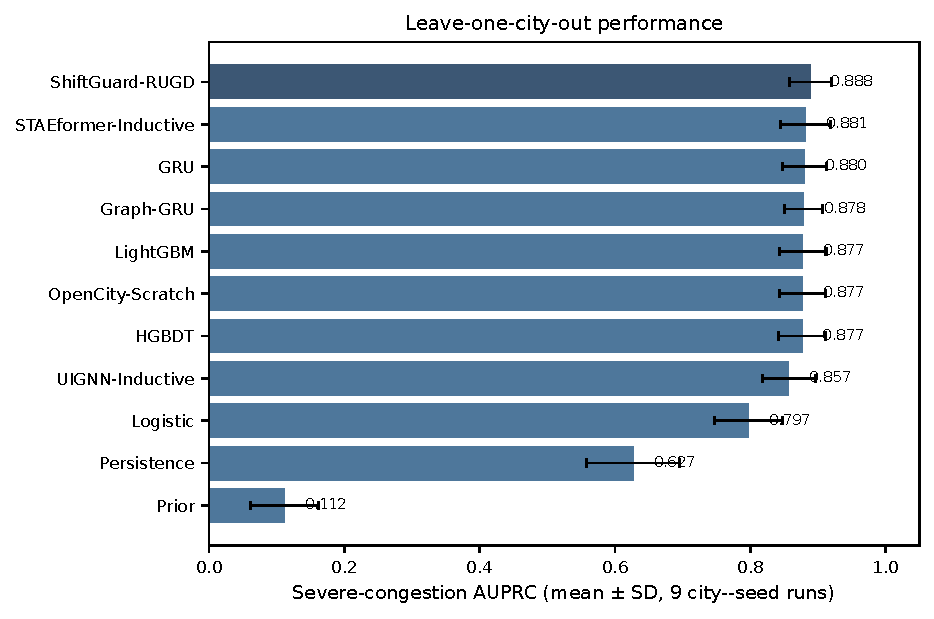
\includegraphics[width=0.85\linewidth]{figures/main_severe_auprc.pdf}
\caption{Severe-congestion AUPRC across all 11 compared models, mean $\pm$ SD over nine
city--seed runs. Source: \texttt{outputs/studies/final\_study/main/results\_all.csv}; rendered by
\texttt{paper/figures/render\_figures.py} from \texttt{paper/figures/data/main\_severe\_auprc.csv}.}
\label{fig:main-auprc}
\end{figure}

\subsection{Robustness under distribution shift}
\label{sec:results-robustness}

% Source: outputs/studies/final_study/main/robustness_all.csv, missingness rows only
% (full 7-condition table is tables/full_robustness.tex in the appendix).
% Regenerate with: python paper/tables/generate_tables.py
\begin{table}[t]
\centering
\caption{Severe AUPRC under 30\% and 50\% independently-masked sensor observations, mean $\pm$ SD over nine city--seed runs; clean-fit source calibration is reused (not re-tuned per condition). Bold marks the best mean per column. See \Cref{app:robustness-full} for all seven registered corruption conditions.}
\label{tab:robustness}
\resizebox{\linewidth}{!}{%
\begin{tabular}{lcc}
\toprule
Method & 30\% missing & 50\% missing \\
\midrule
\textbf{ShiftGuard-RUGD} & 0.7938$\pm$0.0532 & 0.7242$\pm$0.0718 \\
STAEformer-Inductive & \textbf{0.8139$\pm$0.0630} & \textbf{0.7459$\pm$0.0878} \\
Graph-GRU & 0.7408$\pm$0.0953 & 0.5421$\pm$0.2060 \\
GRU & 0.6900$\pm$0.0806 & 0.4734$\pm$0.1359 \\
OpenCity-Scratch & 0.6461$\pm$0.1285 & 0.3784$\pm$0.1885 \\
LightGBM & 0.5597$\pm$0.1253 & 0.3551$\pm$0.1289 \\
HGBDT & 0.5470$\pm$0.1345 & 0.3447$\pm$0.1334 \\
Persistence & 0.4750$\pm$0.0659 & 0.3703$\pm$0.0610 \\
UIGNN-Inductive & 0.7395$\pm$0.0509 & 0.6247$\pm$0.0597 \\
Logistic & 0.3164$\pm$0.0612 & 0.2192$\pm$0.0538 \\
Prior & 0.1117$\pm$0.0505 & 0.1117$\pm$0.0505 \\
\bottomrule
\end{tabular}}
\end{table}


Missing sensors expose \methodname{}'s clearest limitation: STAEformer-Inductive ranks first at
both 30\% and 50\% masking (\Cref{tab:robustness}), while \methodname{} is second, exceeding every
other learned baseline by a wide margin (e.g., +5.30 and +18.20 points over Graph-GRU at 30\%/50\%).
Under strong measurement noise and temporal shift, rankings are closer and no method dominates
every metric (\Cref{fig:robustness}; full seven-condition table in \Cref{app:robustness-full}).

\begin{figure}[t]
\centering
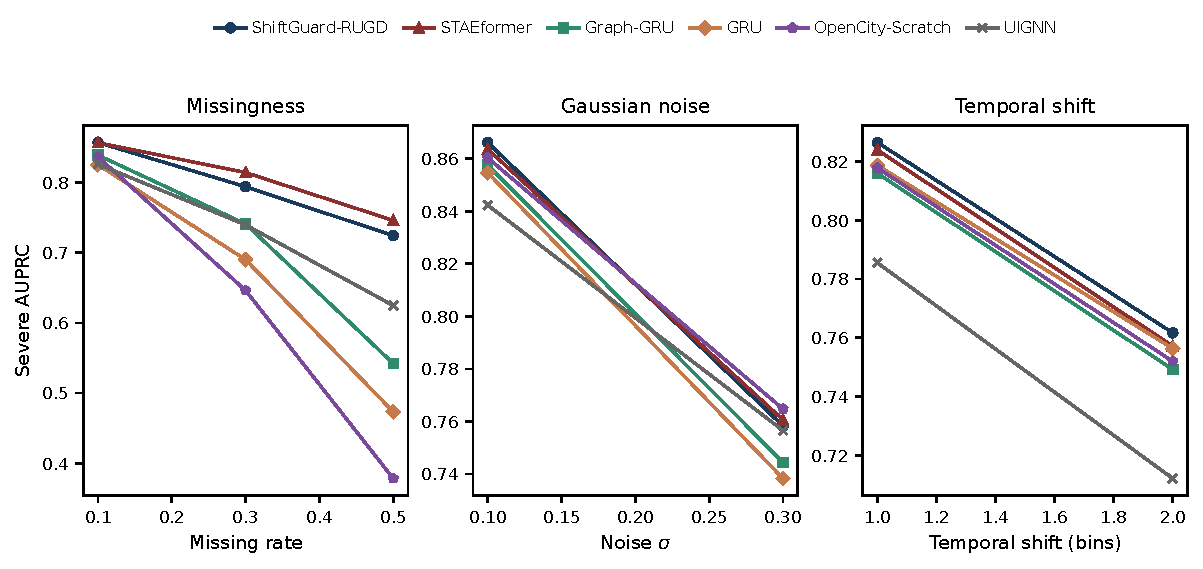
\includegraphics[width=\linewidth]{figures/robustness.pdf}
\caption{Severe AUPRC across all registered corruption severities for a six-model focus set.
Source: \texttt{outputs/studies/final\_study/main/robustness\_all.csv}; rendered by
\texttt{paper/figures/render\_figures.py}.}
\label{fig:robustness}
\end{figure}

\subsection{Component ablations localize the transfer mechanism}
\label{sec:ablations}

% Source: outputs/studies/final_study/ablations/results_all.csv, aggregated per
% variant over nine city-seed runs each.
% Regenerate with: python paper/tables/generate_tables.py
\begin{table}[t]
\centering
\caption{Final-architecture ablations, mean $\pm$ SD over nine city--seed runs each. $\Delta$ is clean severe-AUPRC change from full \methodname{}; bold marks the single largest-magnitude $\Delta$. Domain alignment's removal costs roughly $4\times$ the next-largest component effect (graph diffusion) and roughly $30\times$ the rare-event-specific mechanisms (class balance, evidence).}
\label{tab:ablation}
\begin{tabular}{lccccc}
\toprule
Variant removed & Macro-F1 & Clean severe AUPRC & $\Delta$ & NLL & ECE \\
\midrule
w/o graph diffusion & 0.8325$\pm$0.0128 & 0.8795$\pm$0.0336 & -0.0088 & 0.2714 & 0.0076 \\
w/o topology & 0.8308$\pm$0.0134 & 0.8786$\pm$0.0352 & -0.0097 & 0.2730 & 0.0079 \\
w/o domain alignment & 0.8221$\pm$0.0129 & 0.8538$\pm$0.0403 & \textbf{-0.0344} & 0.3024 & 0.0128 \\
w/o evidence & 0.8357$\pm$0.0113 & 0.8874$\pm$0.0314 & -0.0009 & 0.2632 & 0.0067 \\
w/o focal modulation & 0.8374$\pm$0.0117 & 0.8842$\pm$0.0288 & -0.0041 & 0.2698 & 0.0098 \\
w/o class balance & 0.8367$\pm$0.0116 & 0.8872$\pm$0.0320 & -0.0011 & 0.2626 & 0.0061 \\
\midrule
\textbf{Full ShiftGuard-RUGD} & \textbf{0.8381}$\pm$0.0112 & \textbf{0.8883}$\pm$0.0310 & --- & 0.2625 & 0.0066 \\
\bottomrule
\end{tabular}
\end{table}


\Cref{tab:ablation} and \Cref{fig:ablation-waterfall} give this paper's central, falsifiable
claim: removing domain-adversarial source alignment costs 3.44 severe-AUPRC points -- roughly
$4\times$ the next-largest component effect (graph diffusion, 0.88 points; transferable topology,
0.97 points) and roughly $30\times$ the two rare-event-specific mechanisms (class balancing,
$-0.11$ points; evidential supervision, $-0.09$ points, both within noise of zero). This is not
distributed credit across the architecture: the mechanism doing the heavy lifting for zero-shot
transfer specifically is the explicit cross-city domain-invariance pressure, not the spatial
diffusion or the rare-event machinery, both of which matter far more modestly. Class-balance and
evidential-head removals are, on this three-city sample, negative results -- essentially
noise-level -- and we report them as such rather than retrofit a story where every component
contributes comparably.

\begin{figure}[t]
\centering
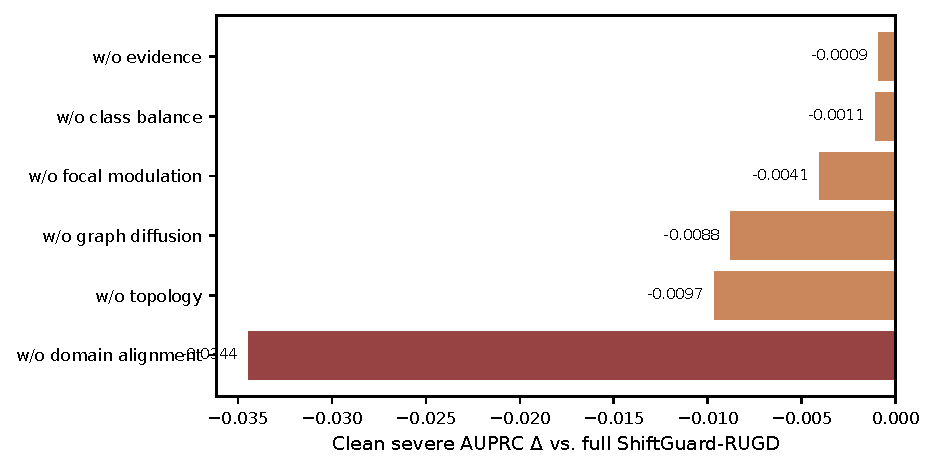
\includegraphics[width=0.85\linewidth]{figures/ablation_waterfall.pdf}
\caption{Clean severe-AUPRC change from removing each component, full \methodname{} as the
reference. Domain alignment dominates. Source:
\texttt{outputs/studies/final\_study/ablations/results\_all.csv}; rendered by
\texttt{paper/figures/render\_figures.py}.}
\label{fig:ablation-waterfall}
\end{figure}

\subsection{Per-city results}
\label{sec:results-percity}

TrafficHZ is the strongest case for \methodname{} (\Cref{tab:percity} in \Cref{app:percity-detail}:
0.8524 macro-F1, 0.9281 severe AUPRC). TrafficCD is a near-tie with STAEformer-Inductive and should
not be presented as a
decisive city-level result; TrafficSH shows a larger clean advantage over the attention-based
adaptations but the lowest absolute severe AUPRC of the three cities.

\subsection{Calibration and efficiency}
\label{sec:results-calib-eff}

\methodname{} has the best NLL and Brier score in the suite but not the best ECE (STAEformer is
lower); full calibration and parameter/throughput tables are in \Cref{app:calibration,app:efficiency}.
APS conformal coverage is 0.9984$\pm$0.0003 against a nominal 0.90 target with mean set size
2.1552$\pm$0.0834 -- substantially over-conservative, and, because source-calibration and an unseen
target city are not guaranteed exchangeable, we report this as an observed transfer result rather
than a formal coverage guarantee. \methodname{} is the smallest neural model in the suite
(38{,}048--66{,}600 parameters, 3--12$\times$ fewer than STAEformer-Inductive) and runs inference
roughly 3.5$\times$ faster than it, while training roughly 2$\times$ faster; it is slower to train
than the plain recurrent controls, since the diffusion, gating, and domain-adversarial machinery is
not free (\Cref{app:efficiency}). The confusion matrix and severe-event calibration/PR curves for
one registered run are given in \Cref{app:qualitative}: errors concentrate between adjacent
severity classes, consistent with the ordinal structure of the label space.
